\chapter{Enhancing D-COACH for High-Dimensional State Problems}
\section{Overview}

In this chapter we introduce  D-COACH ON, a variation of D-COACH OFF for problems with high-dimensional state spaces. This is motivated by the limitation that D-COACH OFF presents when learning state representations. Recording a database with observations of the environment and training an autoencoder in an offline step can be time consuming and not robust to changes in the environment. Thus, it would be desirable to have a version of D-COACH that eliminates this offline step, learning everything in a single interaction step, as the original COACH does. Hence, an algorithm capable of training all the parameters of the network interactively from scratch. 

\section{Online State Representation Learning}
In order to obtain an algorithm capable of learning interactively from scratch we need to make the networks to converge faster. In the former chapter, an autoencoder was used to learn a low-dimensional representation of high-dimensional states in an offline learning process. In this chapter, we propose to use the autoencoder learning criteria during the interactive learning process, such that both networks (the policy and the autoencoder) share the convolutional layers of the encoder, as shown in Fig.~\ref{fig:msim}.

\begin{figure}[H]
    \centering
    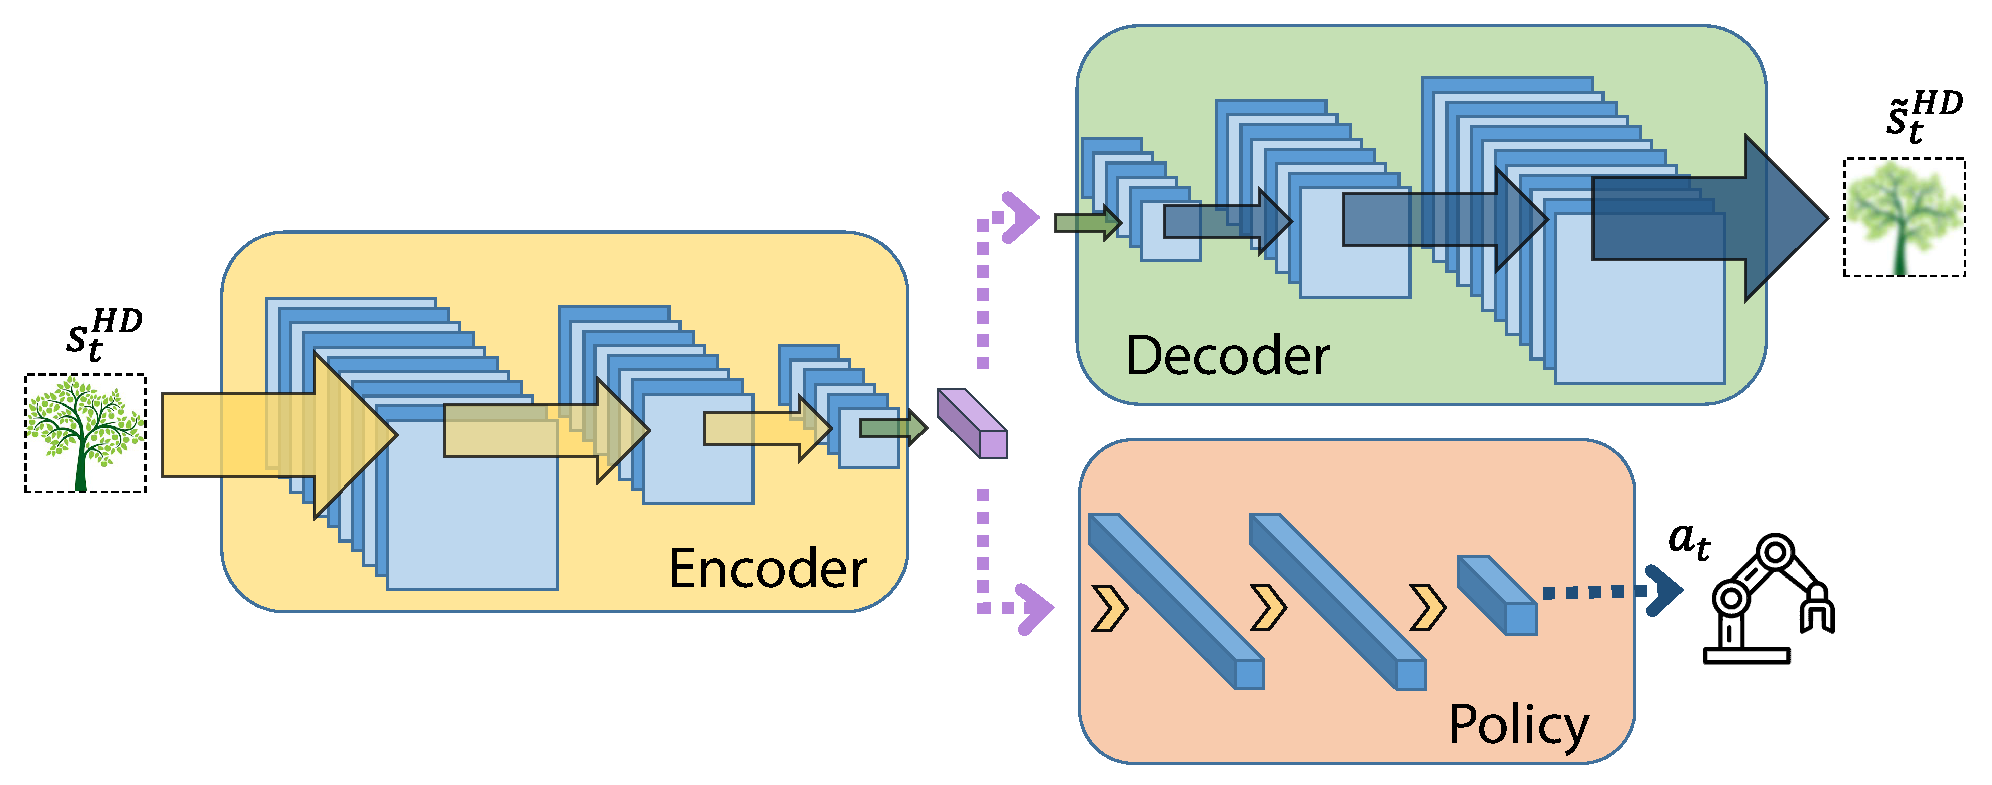
\includegraphics[width=\linewidth]{imagenes/cap2/m2.pdf}
    \caption[D-COACH ON learning scheme.]{D-COACH ON learning scheme. The state representation is shared between the autoencoder and the policy training.}
    \label{fig:msim}
\end{figure}

The policy network has convolutional layers at the input (\emph{Encoder}), followed by a second part that has fully-connected layers (\emph{Policy}). For simplicity, only the layers that are specialized in the decision making are referred as the policy; thus, the fully-connected layers. This network, \emph{Encoder} + \emph{Policy}, maps $s_{t}^{HD}$ into $a_{t}$, while the autoencoder network, \emph{Encoder} + \emph{Decoder}, involves the computation from $s_{t}^{HD}$ to $\widetilde s_{t}^{HD}$, wherein $\widetilde s_{t}^{HD}$ is the reconstructed image at the output of the decoder. Autoencoding is seen as an additional auxiliary criteria for training the state representation of the policy. So, in addition to the loss function for predicting the policy based on the data generated by the human corrections, it also includes the loss function of the reconstruction at the output of the autoencoder, based on the same data stored during the human corrections.

As it can be observed, the structure of the network presented in Chapter 3 is maintained, but the training strategy is modified. 

\section{The Algorithm}
Algorithm \ref{algorithm:EnDeepCOACH} describes D-COACH ON. The algorithm first sets the hyper-parameters like the magnitude of the error (Equation \ref{eq:error}), and the ones used for the corrections replay. In cases when the teacher advises a correction (line 6, Algorithm \ref{algorithm:EnDeepCOACH}), the subsequent lines are evaluated, wherein the policy network is updated along with the autoencoder network.

Two different updates are computed, one for the layers involved in the policy computation, and another for the layers of the autoencoder. When feedback is given by the teacher, the \textbf{update} \emph{policy} instruction updates the policy network for the current time step only using this last received feedback. Subsequently, the \emph{batch\_update} subroutine is called. This subroutine is in charge of updating the policy and the autoencoder by sampling a mini-batch from the replay buffer. The \emph{batch\_update} subroutine is also called every $b$ time steps (line 15, Algorithm \ref{algorithm:EnDeepCOACH}).

The \emph{batch\_update} subroutine is described in Algorithm \ref{algorithm:batch_update}. When this subroutine is called, the autoencoder is updated only if its reconstruction error in the last \emph{m} observations (MSE between  $s_{t}^{HD}$ and $\widetilde s_{t}^{HD}$) is greater than a threshold $\epsilon$ (line 4, Algorithm \ref{algorithm:batch_update}), which is determined empirically such that the autoencoder learns to generate good representations of the input before freezing its layers. Otherwise, the autoencoder is not updated and the convolutional layers of the encoder are frozen. As a consequence, the instruction \textbf{update} \emph{policy} in lines 3 (Algorithm \ref{algorithm:batch_update}) and 10 (Algorithm \ref{algorithm:EnDeepCOACH}) only modifies the non-convolutional layers of the policy. 

The condition for training the autoencoder is used for avoiding conflicts in the gradients of both cost functions, so when the latent vector of the autoencoder is considered a good smaller representation of the state, the gradient of the policy must be prevented from harming the learned encoding. Hence, the encoder is kept frozen, unless unknown regions of the state space are visited. 

\begin{algorithm}[h]
\caption{D-COACH ON: Online State Representation Learning}\label{algorithm:EnDeepCOACH}
\begin{algorithmic}[1]
\algdef{SE}[SUBALG]{Indent}{EndIndent}{}{\algorithmicend\ }%
\algtext*{Indent}
\algtext*{EndIndent}

\State \textbf{Require:} error magnitude $\textit{e}$, buffer update interval $b$, buffer sampling size $N$, buffer max. size $K$, buffer min. size $k$, sequence length for AE reconstruction error \emph{m}, AE reconstruction error threshold $\epsilon$, pre-trained encoder parameters (if 3-step sequential learning) 
\State \textbf{Init:} $\mathcal{B} = []$ \emph{\# initialize memory buffer}
\For{t = 1,2,...}{} \emph{\# main loop}
\State \textbf{observe} state $s_{t}$
\State \textbf{execute} action $a_{t}=\pi(s_{t})$
\State \textbf{feedback} human corrective advice $h_{t}$
\If{$h_{t}$ is not \textbf{0}}
\State $\mathrm{error}_{t} = h_{t}\cdot e$
\State $y_{\mathrm{label}(t)} = a_{t} + \mathrm{error}_{t}$ 
\State \textbf{update} \emph{policy} using SGD with pair ($s_{t}$, $y_{\mathrm{label}(t)}$) 
\State \textbf{call} batch\_update
\State \textbf{append} $(s_{t}, y_{\mathrm{label}(t)})$ to $\mathcal{B}$
\EndIf
\If{length($\mathcal{B}$) $> K$ }
\State $\mathcal{B} = \mathcal{B}[2:K+1]$
\EndIf
\If{$\operatorname{mod}(t, b)$ is 0}
\State \textbf{call} batch\_update
\EndIf
\EndFor
\end{algorithmic}
\end{algorithm}

\begin{algorithm}[h]
\caption{D-COACH ON Subroutine: \emph{batch\_update}}\label{algorithm:batch_update}
\begin{algorithmic}[1]
\algdef{SE}[SUBALG]{Indent}{EndIndent}{}{\algorithmicend\ }%
\algtext*{Indent}
\algtext*{EndIndent}
\State \textbf{function} batch\_update \emph{\# define batch update function}
\Indent
\If{$\mathrm{length}(\mathcal{B}) \geq k$}
\State \textbf{update} \emph{policy} using SGD with a mini-batch sampled from $\mathcal{B}$
\If{$AE_{\mathrm{error}}>\epsilon$}
\State \textbf{unfreeze} convolutional layers
\State \textbf{update} $AE$ using SGD with a mini-batch sampled from $\mathcal{B}$
\Else
\State \textbf{freeze} convolutional layers
\EndIf
\EndIf
\EndIndent
\end{algorithmic}
\end{algorithm}

\section{Experiments and Results}

Three different types of experiments were carried out for validating D-COACH ON: i) experiments with simulated teachers for evaluating the learning method under controlled conditions without influence of human factors, ii) validations with real human teachers, and iii) extra validations on real physical systems.

In the experiments, the learning processes are analyzed in three different problems:

\textbf{(i) Car Racing:} Exactly the same problem as the one used in Chapter 2. The coupled feedback strategy was also used in this case. 
    
\textbf{(ii) Duckie Racing:} Also the same problem as the one used in Chapter 2 with the difference that now also a simulation of this environment was used \cite{gym_duckietown}. The same map was used for both the simulated and real robot. In the simulations, at the beginning of each episode, the robot can start, randomly, at the points A or B (plus random noise) of the map (see Fig.~\ref{fig:duckietown2}). Each simulated episode lasts 1,000 time steps (unless the robot leaves the road before), and as a performance metric a modified version of the default reward function of the environment is used, which is: $R = Cv\theta - Dd$. $C$ and $D$ are constants ($C=100$, $D=1$), $v$ is speed of the duckiebot, $\theta$ is its orientation with respect to $\gamma$ (a bezier curve that defines the path the agent is expected to follow), and \emph{d} is its distance to $\gamma$.

\begin{figure}[h]
\centering
\subfloat[][Duckiebot.]{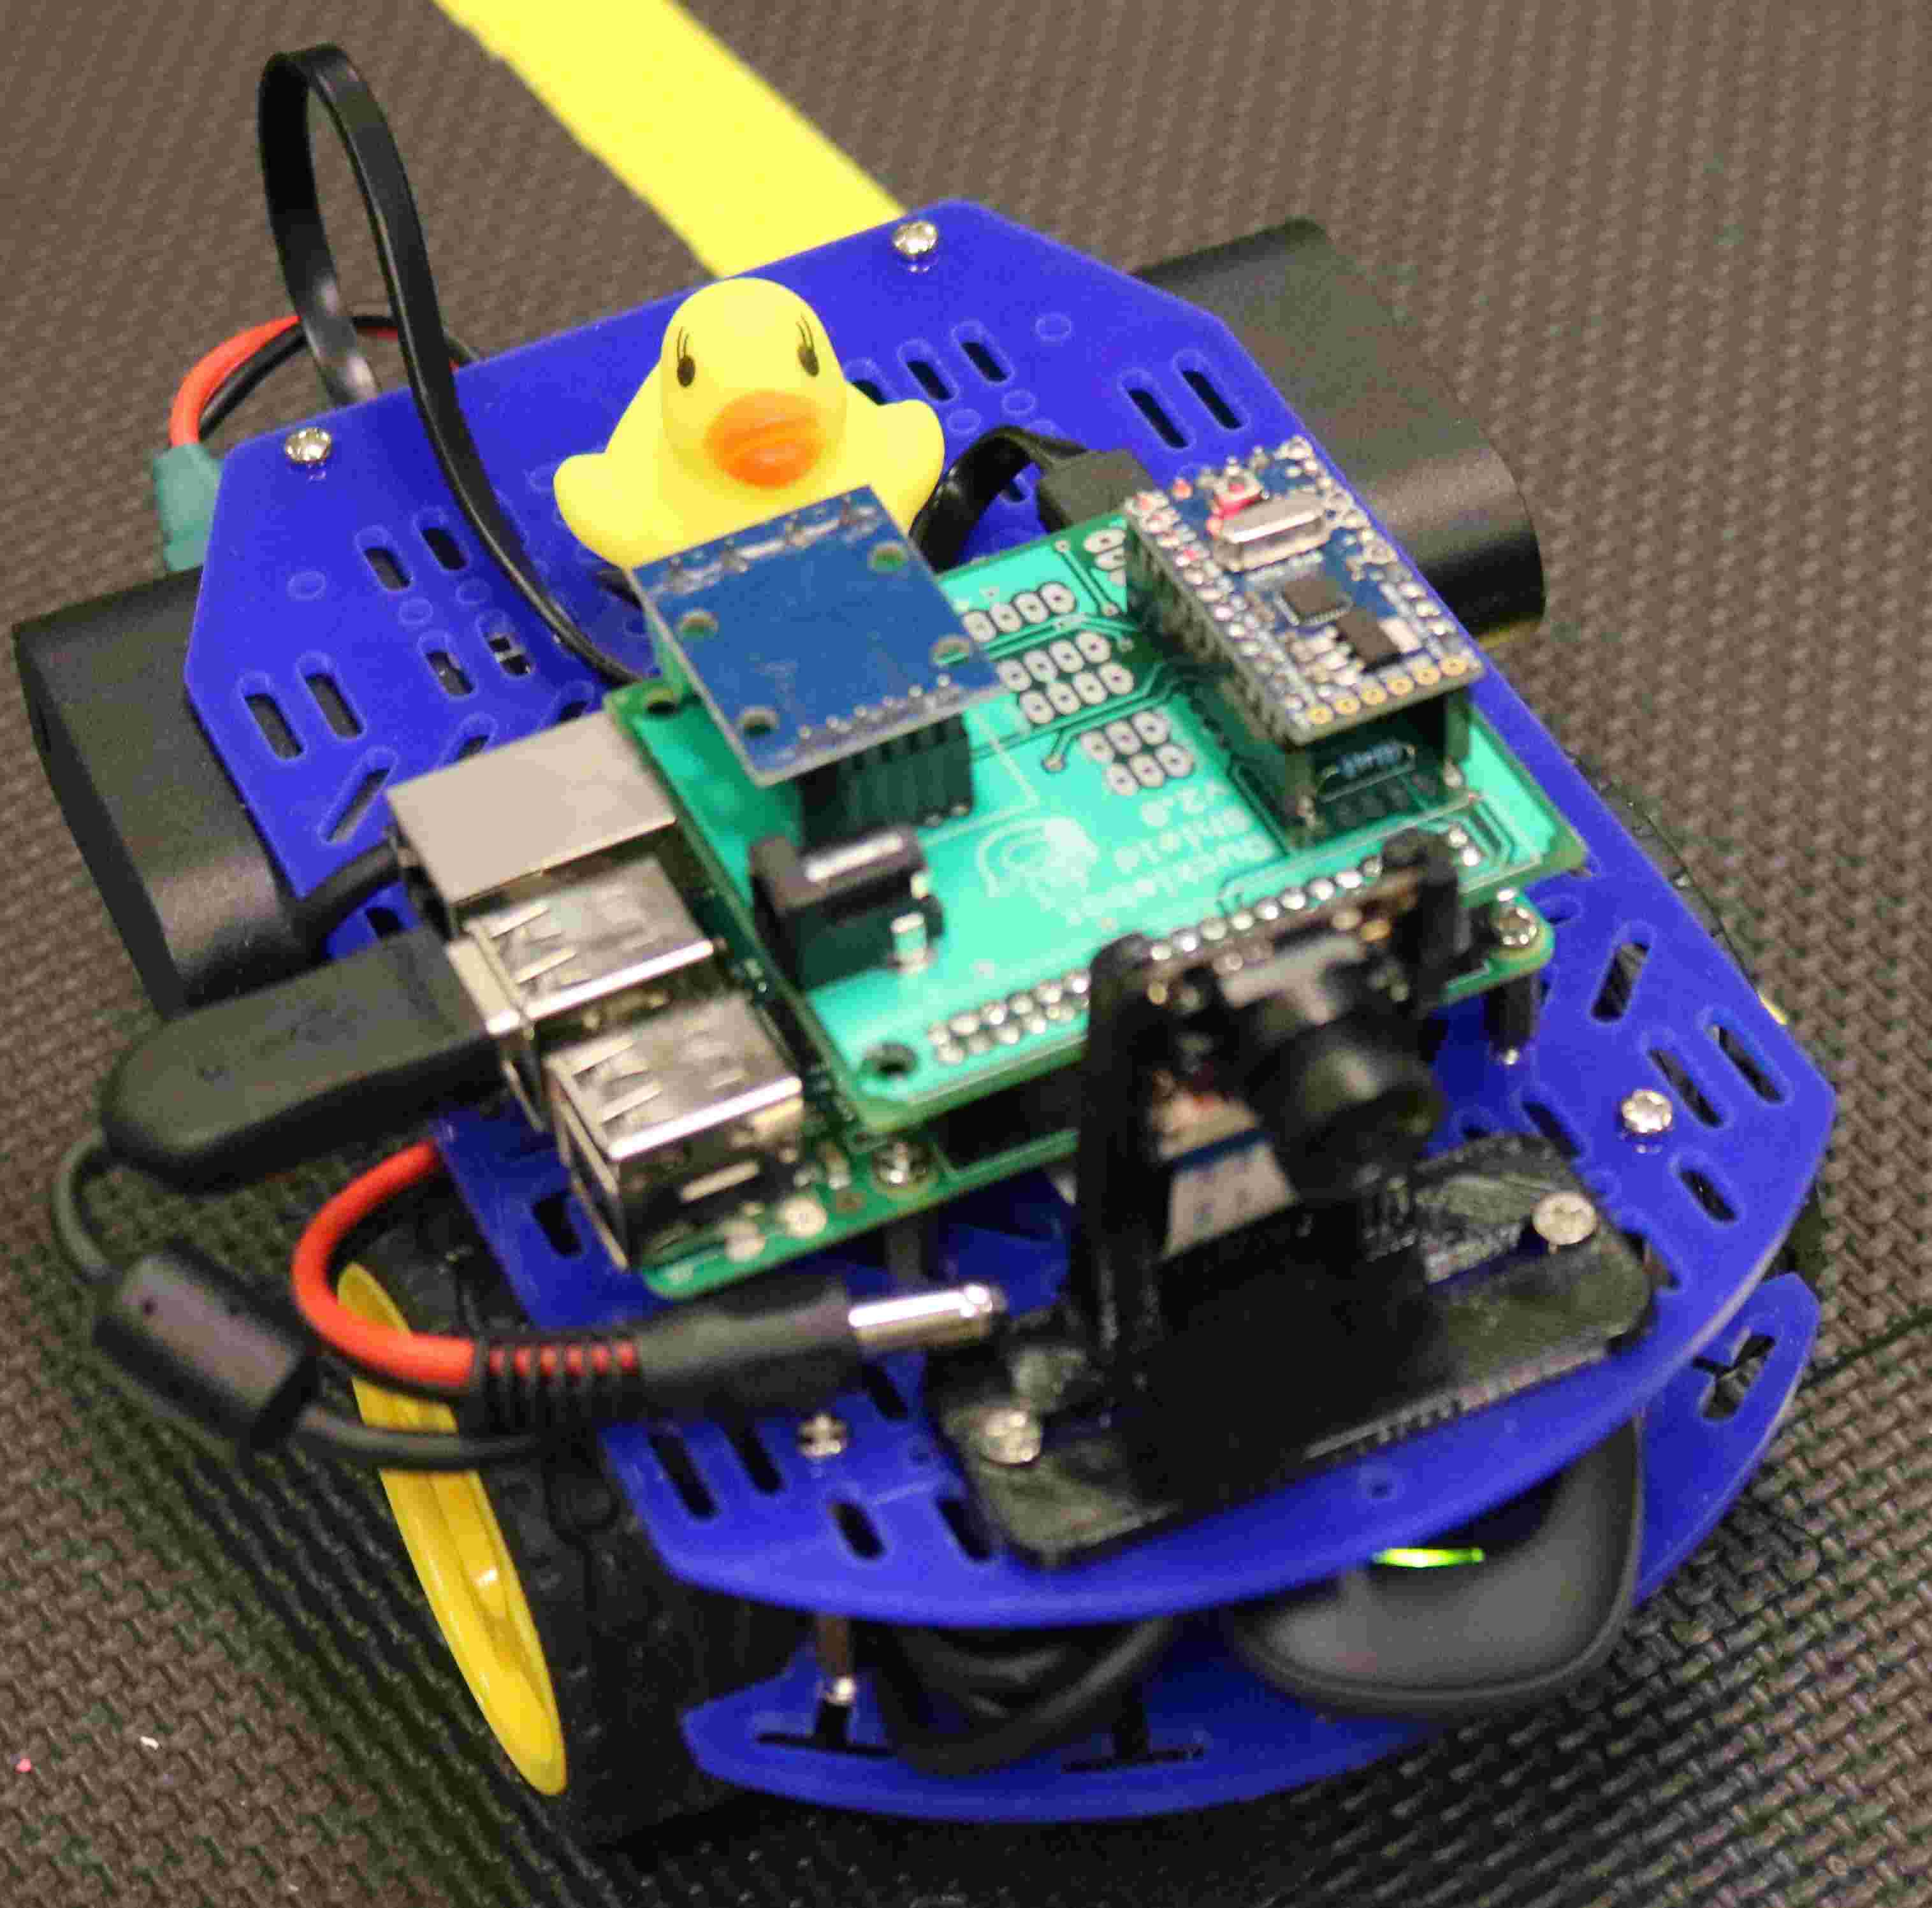
\includegraphics[width=0.23\linewidth]{imagenes/cap3/duckie_image.jpg}}
\hspace{1.1cm}
\subfloat[][First-person view.]{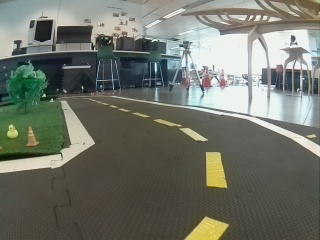
\includegraphics[width=0.3\linewidth]{imagenes/cap3/real_duckie_view.jpg}}
\hspace{4cm}
\subfloat[][Map.]{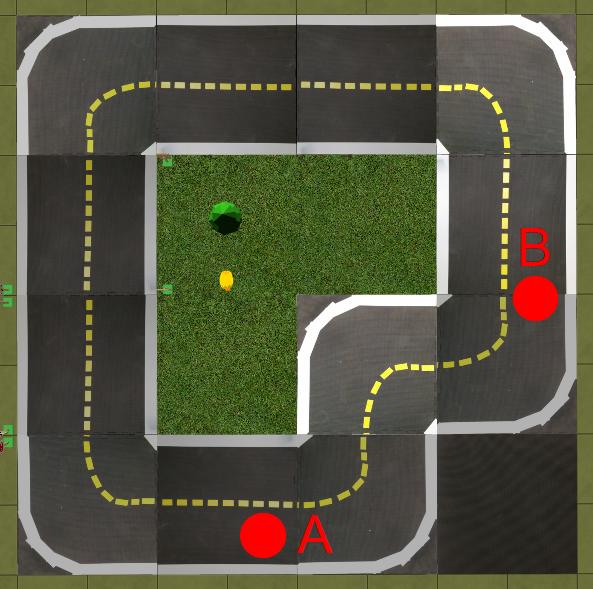
\includegraphics[width=0.23\linewidth]{imagenes/cap3/duckie_map.png}}
\hspace{1.1cm}
\subfloat[][First-person simulated view.]{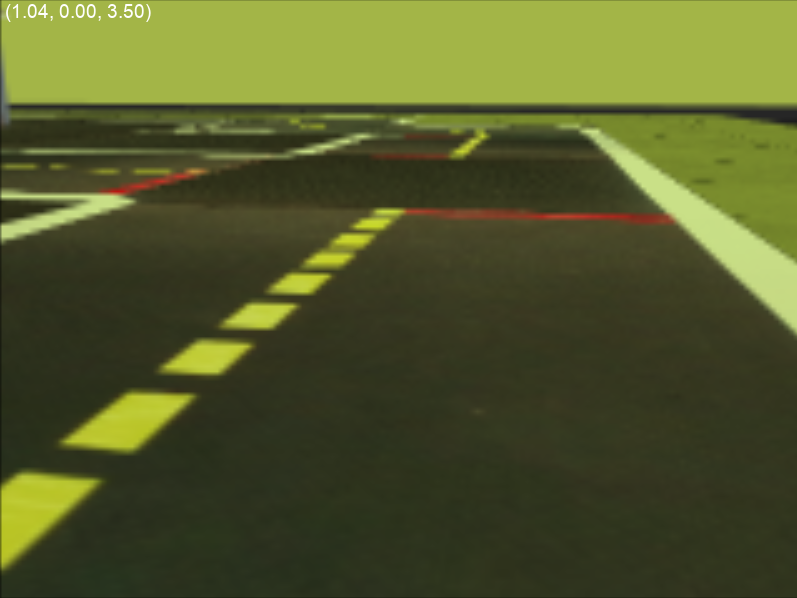
\includegraphics[width=0.3\linewidth]{imagenes/cap3/simplesim_1.png}}
\caption{Duckietown D-COACH OFF.} 
\label{fig:duckietown2} 
\end{figure}

\textbf{(iii) Pusher/Reacher:} Two validation tasks with a 3DoF robotic arm (see Fig.~\ref{fig:PusherReacher}). The problems of pushing  and reaching an object were addressed. For both tasks the robot arm is placed in front of the work-space and an RGB camera is fixed overhead for capturing the top-down view of the environment with images of $640\times480\times3$ size. The images are downsampled to $64\times64\times3$. The objective of the Pusher task is to move the object placed in the work-space down, until it is out, as depicted in Fig.~\ref{fig:PusherReacher}(b). The objective of the Reacher is to track the position of the object with the arm's end effector (Fig.~\ref{fig:PusherReacher}(c)). In these problems, the teacher advises corrections of the position commands of the arm in the Cartesian space. The experiments of the tasks with the 3DoF robot arm were intended only to validate the proposed learning method in another real setup, no comparisons were carried out. These experiments were done at TU Delft by Carlos Celemin, as a part of the paper \emph{"Continuous Control for High-Dimensional State Spaces: An Interactive Learning Approach"} \cite{perez2019continuous}, which is mentioned in the Appendix.

\begin{figure}[h]
\centering
\subfloat[][3DoF robot arm.]{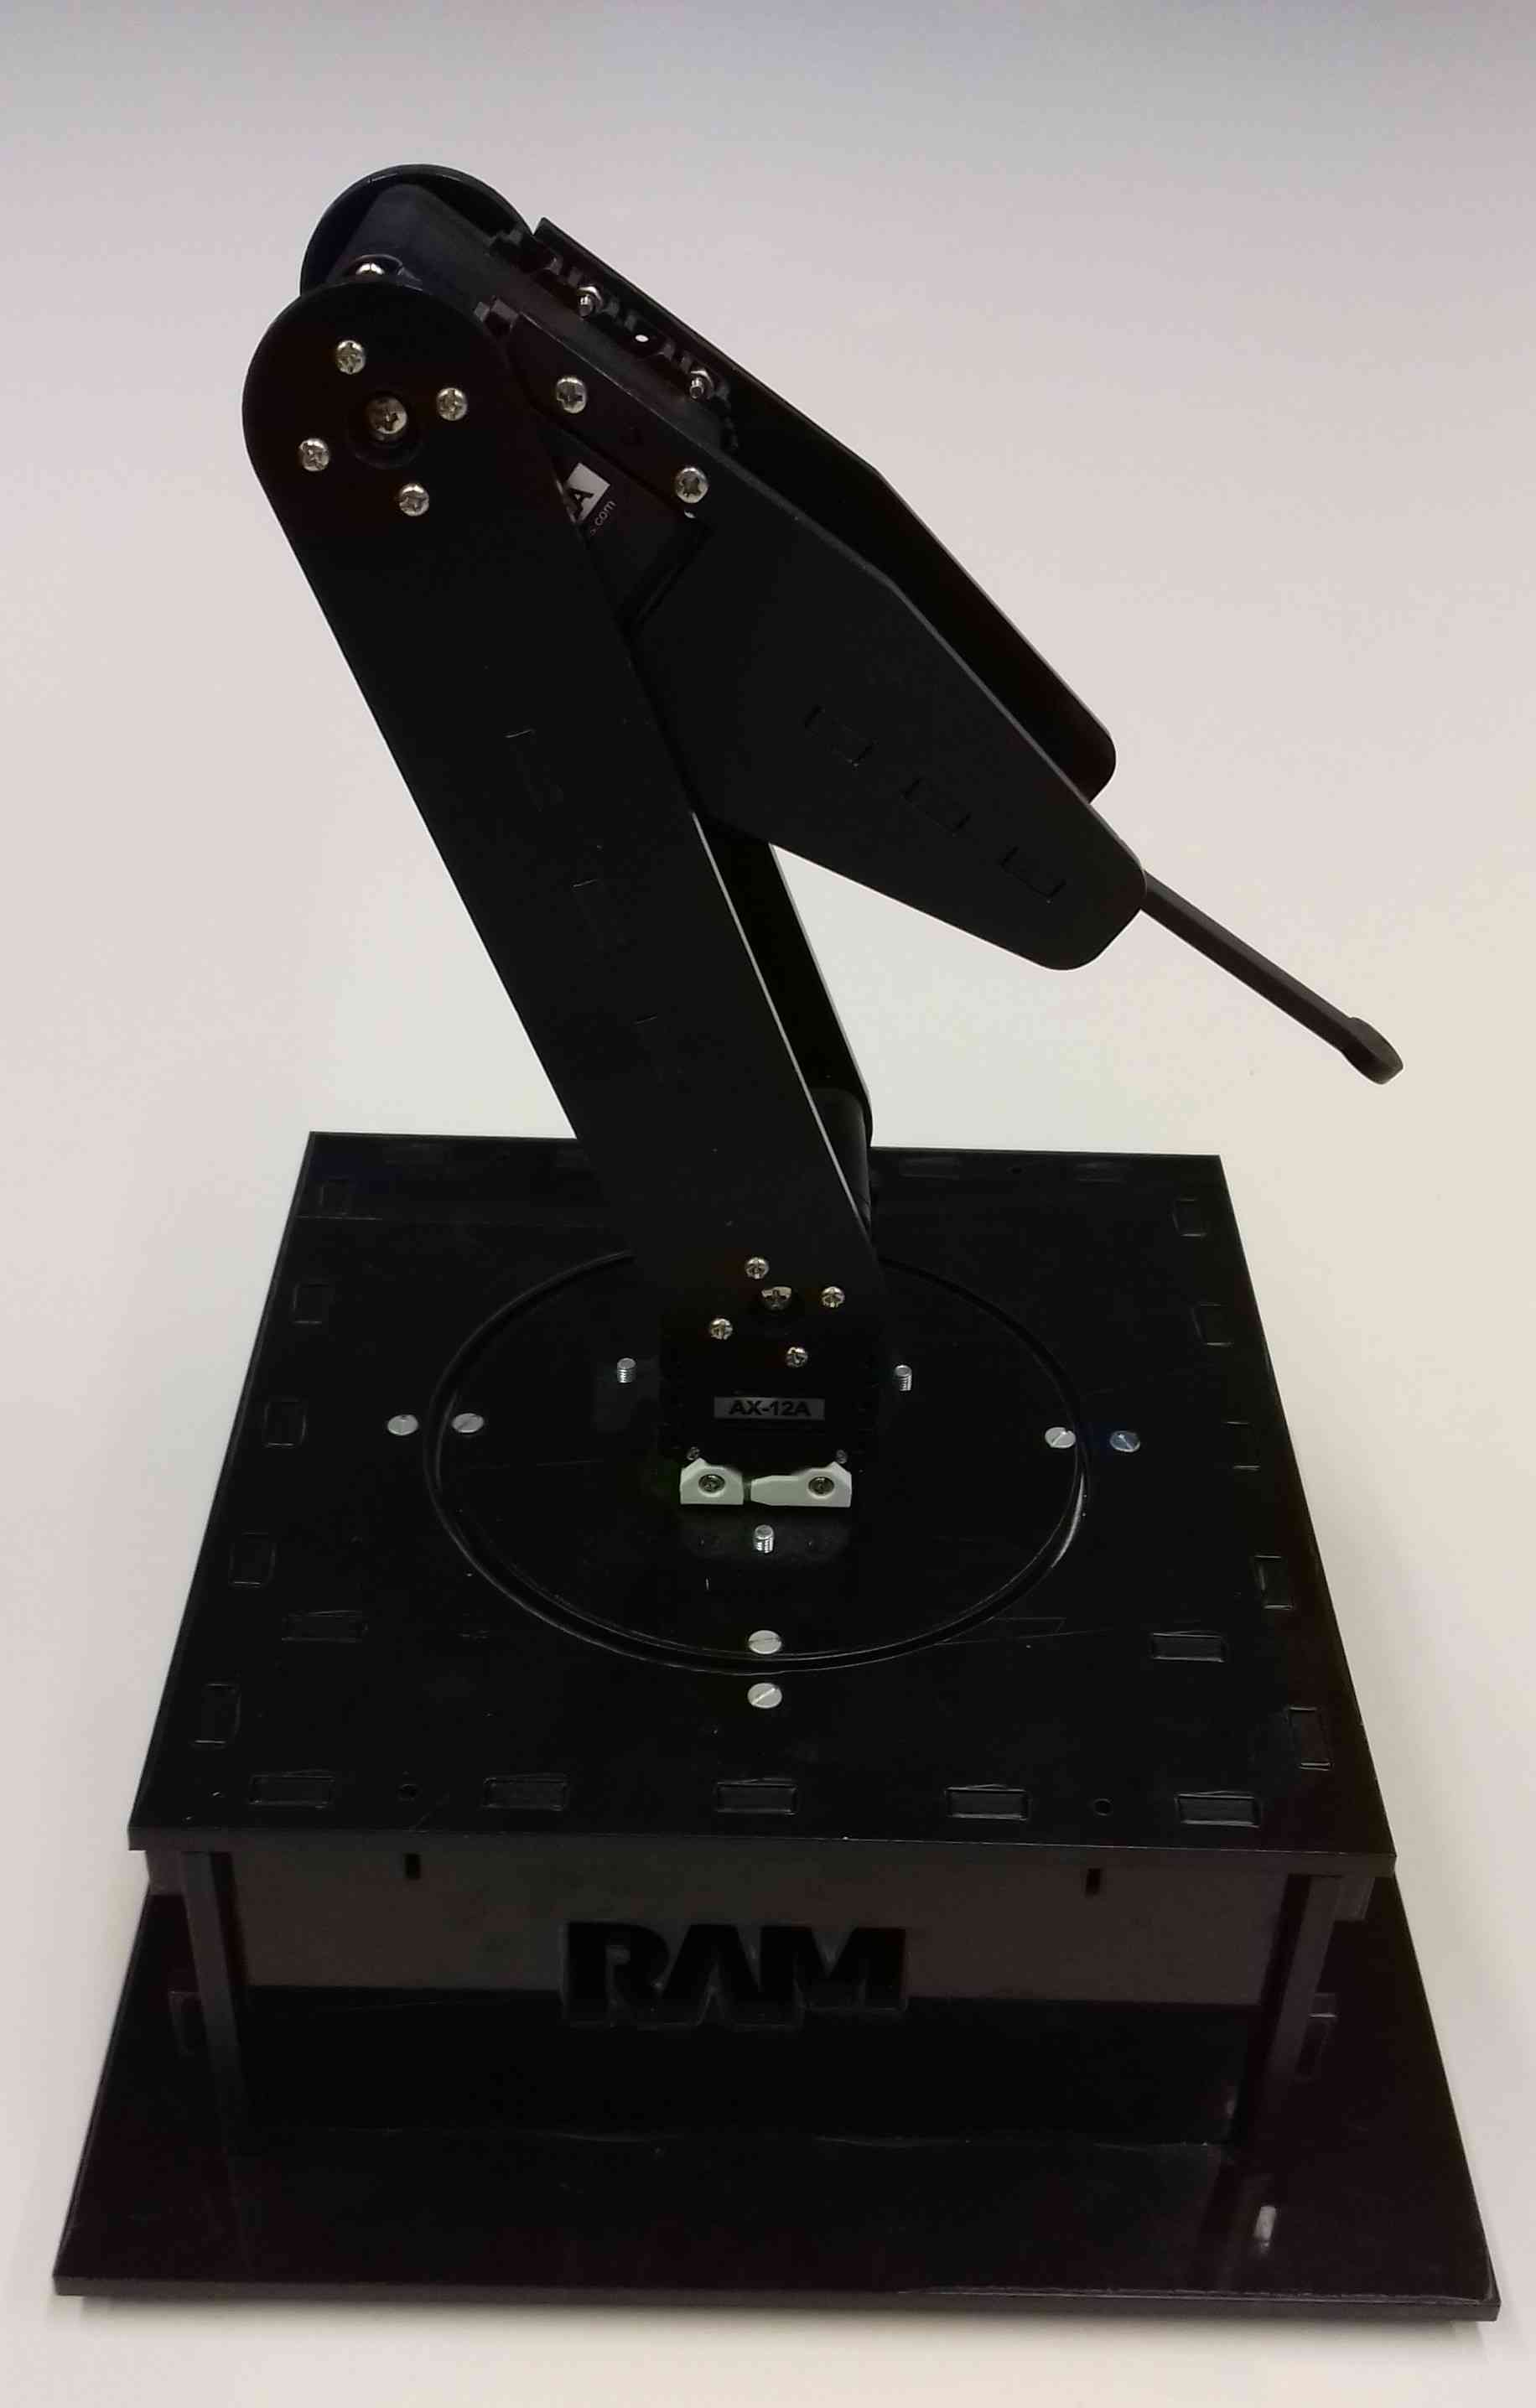
\includegraphics[width=0.2\linewidth]{imagenes/cap3/3dofarm2.jpg}} 
\hspace{0.25cm}
\subfloat[][Pusher task.]{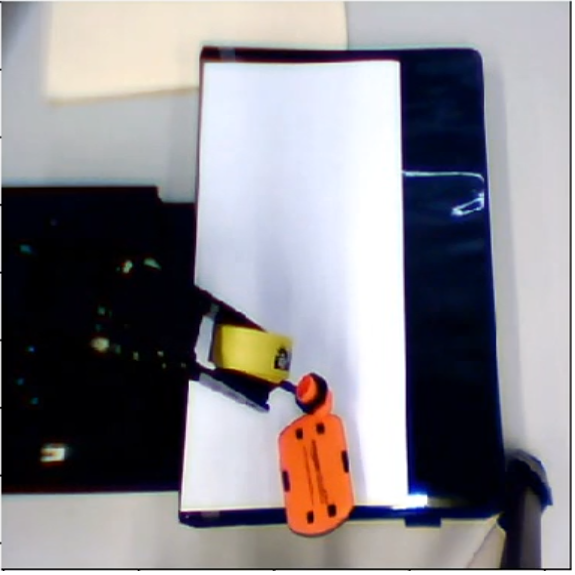
\includegraphics[width=0.315\linewidth]{imagenes/cap3/pusher.png}} 
\hspace{0.25cm}
\subfloat[][Reacher task.]{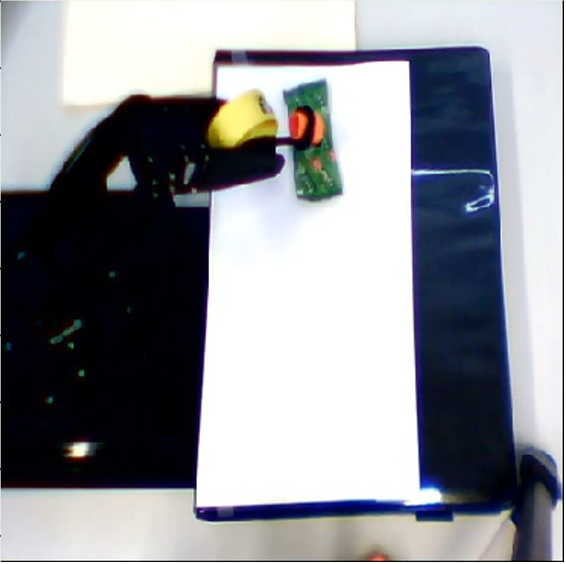
\includegraphics[width=0.315\linewidth]{imagenes/cap3/reacher.png}}
\hspace{0.25cm}
\caption{Pusher/Reacher.} 
\label{fig:PusherReacher} 
\end{figure}

All the results that present averaged data in the form of a curve have confidence intervals that represent the $60^{th}$ percentile of the data.
The neural network hyper-parameters used in Chapter 3 were also used in this chapter (Figure \ref{fig:network_diagram} and Tables \ref{table:off_hypers1}, \ref{table:off_hypers2} and \ref{table:off_hypers3}, ignoring the Cart-Pole hyperparameters and using the size of the state space and action space of the 3DoF arm as the input size and output size of the network used for the reacher and pusher tasks).The experiments are illustrated in the following video \url{https://youtu.be/i4f1D4CH26E}. 

\subsection{Study with Simulated teacher}
In order to evaluate the method along with subtle variants under more controlled conditions, a high performance policy standing-in as a teacher, which was actually trained with $\text{D-COACH ON}$ and a real human teacher, was used (in the same way as in Chapter 2).

To perform an ablation study that evaluates the contribution of the new components of D-COACH ON, the complete method (D-COACH ON A, Algorithm \ref{algorithm:EnDeepCOACH}) is compared to a second variant that includes the AE cost function, but never freezes the convolutional layers (D-COACH ON B), so it always modifies the parameters of the complete policy network using the gradient of both cost functions (i.e. setting $\epsilon=0$ for the condition in line 6). 

The third evaluated variant does not include the AE contribution, and learns the whole policy network only with the cost of predicting the action (D-COACH ON C). This variant works like D-COACH OFF, but skipping the first two steps of recording demonstrations and pre-training the AE, i.e., learning from scratch, which means that the convolutional layers are also learned with the teacher's corrections. The learning curves of the three cases of D-COACH ON are compared against a DDPG-based RL agent \cite{Lillicrap2015} implemented by OpenAI \cite{baselines}. The curves are the average of 30 runs for each case, showing the evolution of the return through the learning time. The time considered is measured when rendering the environments, i.e., no environment acceleration, since D-COACH is intended for learning with real systems wherein speeding up the environment is not possible.

As shown in the Fig.~\ref{fig:simulatedteachers} for the experiments with the Car Racing, the D-COACH ON A and B have a considerable improvement when simultaneously using the gradients of the auto-encoding cost function for learning the state representation, along with the gradient of the policy, in contrast to using only the gradient of the policy (D-COACH ON C), which is slower, and reaches less than $50\%$ of outcome with respect to the complete algorithm after 20 minutes of training. Additionally, there is no noticeable improvement in the performance for the RL agent within this time frame.

\begin{figure}[h]
    \centering
    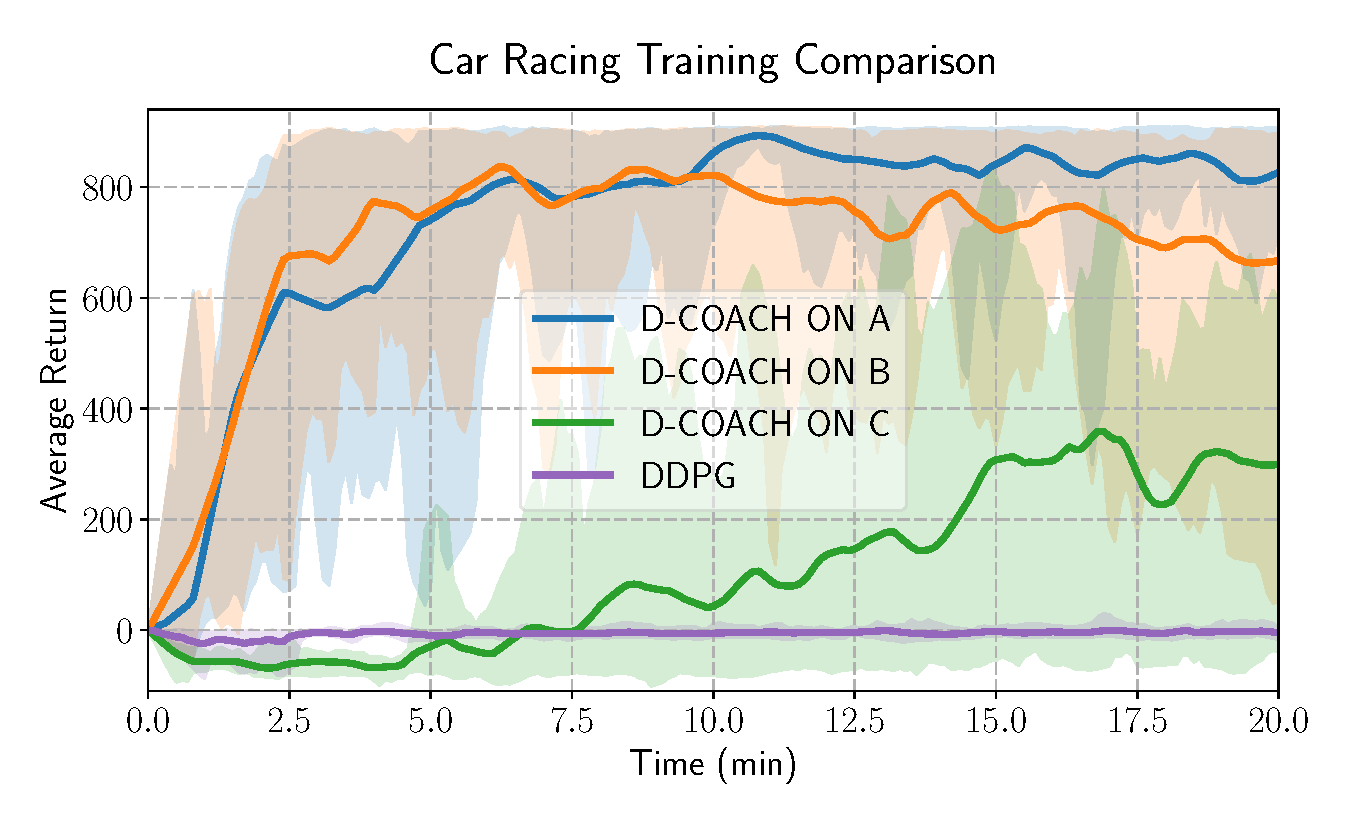
\includegraphics[width=0.7\linewidth]{imagenes/cap3/car_racing_sim_ICRA.pdf}
    \caption[Car Racing results for simulated teacher with D-COACH ON and DDPG.]{Car Racing results for simulated teacher with D-COACH ON and DDPG. D-COACH ON A: policy and AE costs, freezing conv. layers; D-COACH ON B: policy and AE costs; D-COACH ON C: only policy cost. $K = 1000$; $k=20$; $b = 10$; $N = 8$. $P_{h}$: $\alpha = 0.6$; $\tau = 0.000015$; $\emph{e}=\textbf{1}$; $m=50$; $\epsilon=0.0011$. Simulated teacher network learning rate: $0.0003$; Autoencoder learning rate: $0.0003$.}
    \label{fig:simulatedteachers}
\end{figure}

\begin{figure}[h]
    \centering
    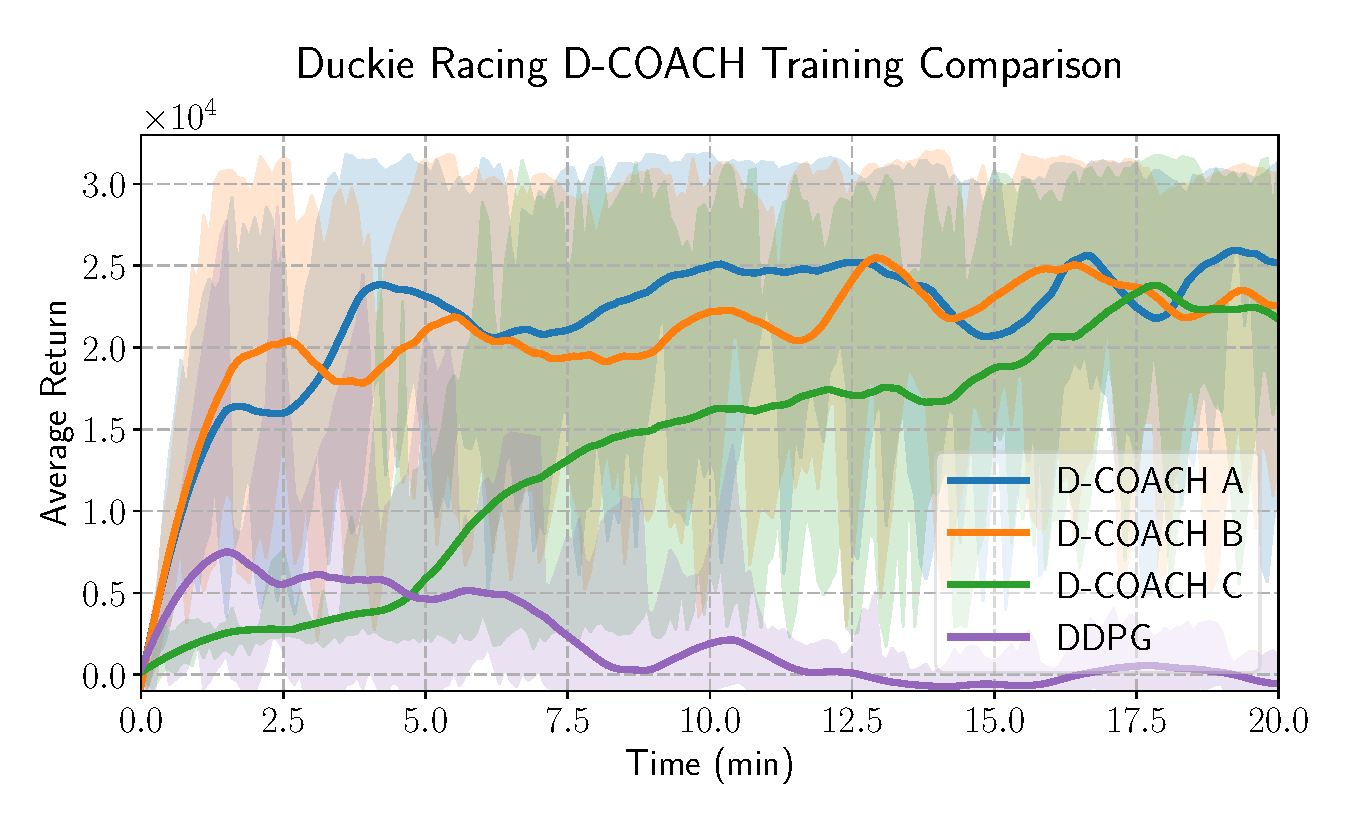
\includegraphics[width=0.7\linewidth]{imagenes/cap3/duckie_sim_ICRA.pdf}
    \caption[Duckie Racing results for simulated teacher with D-COACH ON and DDPG.]{Duckie Racing results for simulated teacher with D-COACH ON and DDPG. D-COACH ON A: policy and AE costs, freezing conv. layers; D-COACH ON B: policy and AE costs; D-COACH ON C: only policy cost. $K = 1000$; $k=20$; $b = 10$; $N = 8$. $P_{h}$: $\alpha = 0.6$; $\tau = 0.000015$; $\emph{e}=\textbf{1}$; $m=50$; $\epsilon=0.0011$.. Simulated teacher network learning rate: $0.0003$; Autoencoder learning rate: $0.0003$.}
    \label{fig:racing_car_results}
\end{figure}

The results of the experiments with the Duckie Racing problem (Fig.~\ref{fig:simulatedteachers}) show similar trends as observed with the Car Racing problem, wherein the contribution of the AE cost function makes a considerable difference with respect to only using the policy cost. However, in this problem, D-COACH ON C manages to reach the same level of performance of the other variants after 17 minutes of training. This variant can learn good policies for this problem, but for reaching $95\%$ of the final performance, it is around 5 times slower than the variants using simultaneous auto-encoding. For this problem again the DDPG learning process does not obtain any improvement during the first 20 minutes of the learning process. 

Finally, it is possible to see the contribution of the condition stated for freezing the convolutional layers, when the error of the decoder is small (D-COACH ON A v/s B). This rule provides more stability to the learning process. In the Car Racing experiments, $\text{D-COACH ON B}$ undergoes an ``unlearning'' stage after 10 minutes of training, whereas in the Duckie Racing experiments is not possible to notice any considerable difference between both approaches. When the error of the decoder is small it means that the latent vector is a good representation of the state, but still the gradient and the error of the policy can be large; therefore, in some cases there may be conflicts that harm the AE performance and consequently the performance of the policy. Freezing these layers is a detail that could solve this conflict.

\subsection{Experiments with real human teachers}

The experiments with simulated teachers are useful for analyzing the evolution of the learning process. However, D-COACH is an interactive learning method; therefore, it is necessary to carry out experiments with real human teachers for complementing its evaluation. Specifically, we perform experiments for measuring the human effort in terms of the time dedicated to teach the agent. The experiments compare D-COACH OFF and D-COACH ON, evaluating the necessary effort (time) to achieve some levels of performance. Ten participants between 20 and 27 years old were asked to act as teachers for both the Car Racing and the Duckie Racing problem. In each problem, the participants corrected the agent's actions with the arrow symbols of a keyboard for a limited session of 20 minutes. 
The average results are presented and discussed.

In Fig.~\ref{fig:stacked_bar} the time dedicated for training the agents is depicted. In the cases of learning with D-COACH OFF, the blue bar indicates the time dedicated by the teachers in its first step of recording demonstrations, which for both problems is actually longer than the time used for reaching the highest level of performance with D-COACH ON. In total, the new method saves around $45\%$ of the training time for the Car Racing problem, and above $80\%$ for the Duckie Racing problem. These results do not include the time dedicated to train the AE in the D-COACH OFF, which would depend on the available hardware. The bar diagram is complemented with the learning curves in Figures ~\ref{fig:humanteachers1} and ~\ref{fig:humanteachers2} (for D-COACH OFF the curve is only after training the AE), wherein it is shown that D-COACH ON has a similar progress with a very slight advantage over its basic version, even without considering the additional time required for the AE training step.

\begin{figure}[H]
\centering
\subfloat[][Car Racing.]{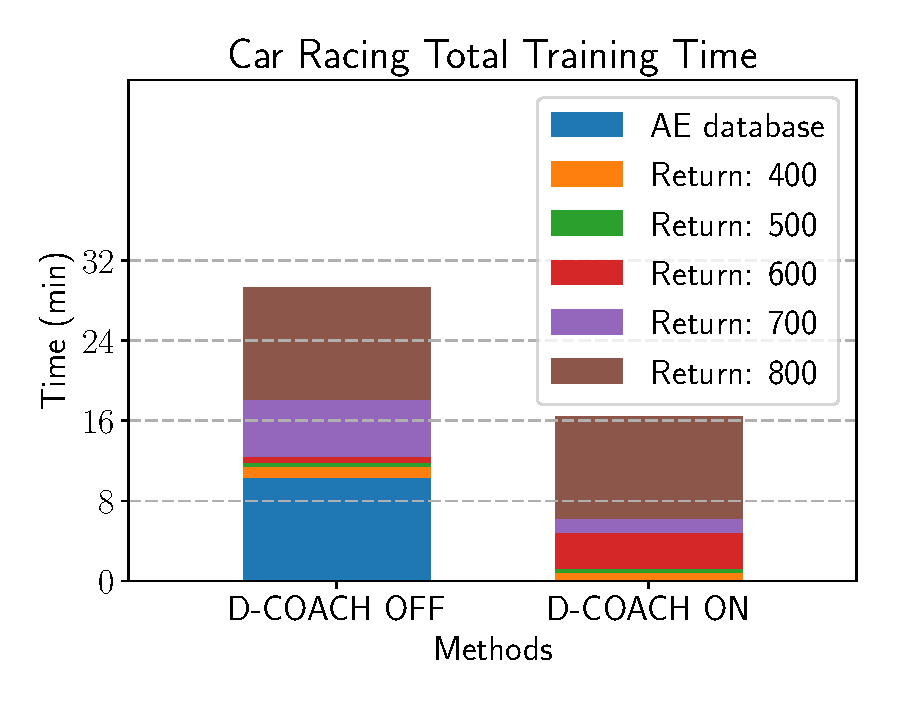
\includegraphics[width=0.4\linewidth]{imagenes/cap3/bar_car_racing_ICRA.pdf}}
\subfloat[][Duckie Racing.]{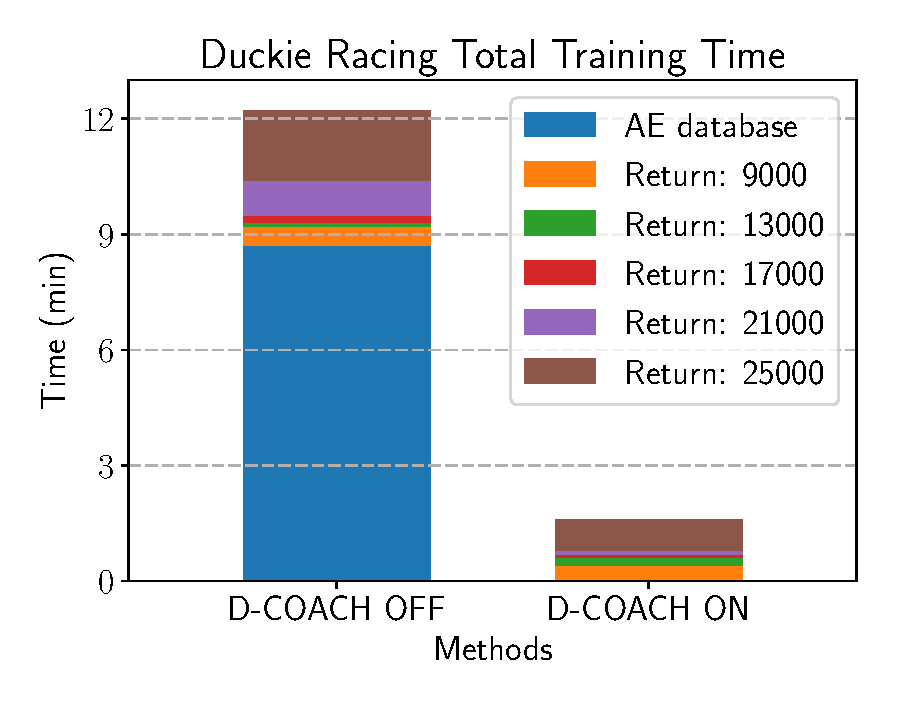
\includegraphics[width=0.4\linewidth]{imagenes/cap3/bar_duckie_ICRA.pdf}}
\caption[Comparison of the average human time dedicated to achieve for the first time some levels of return.]{Comparison of the average human time dedicated to achieve for the first time some levels of return (on average).} 
\label{fig:stacked_bar} 
\end{figure}

\begin{figure}[H]
    \centering
    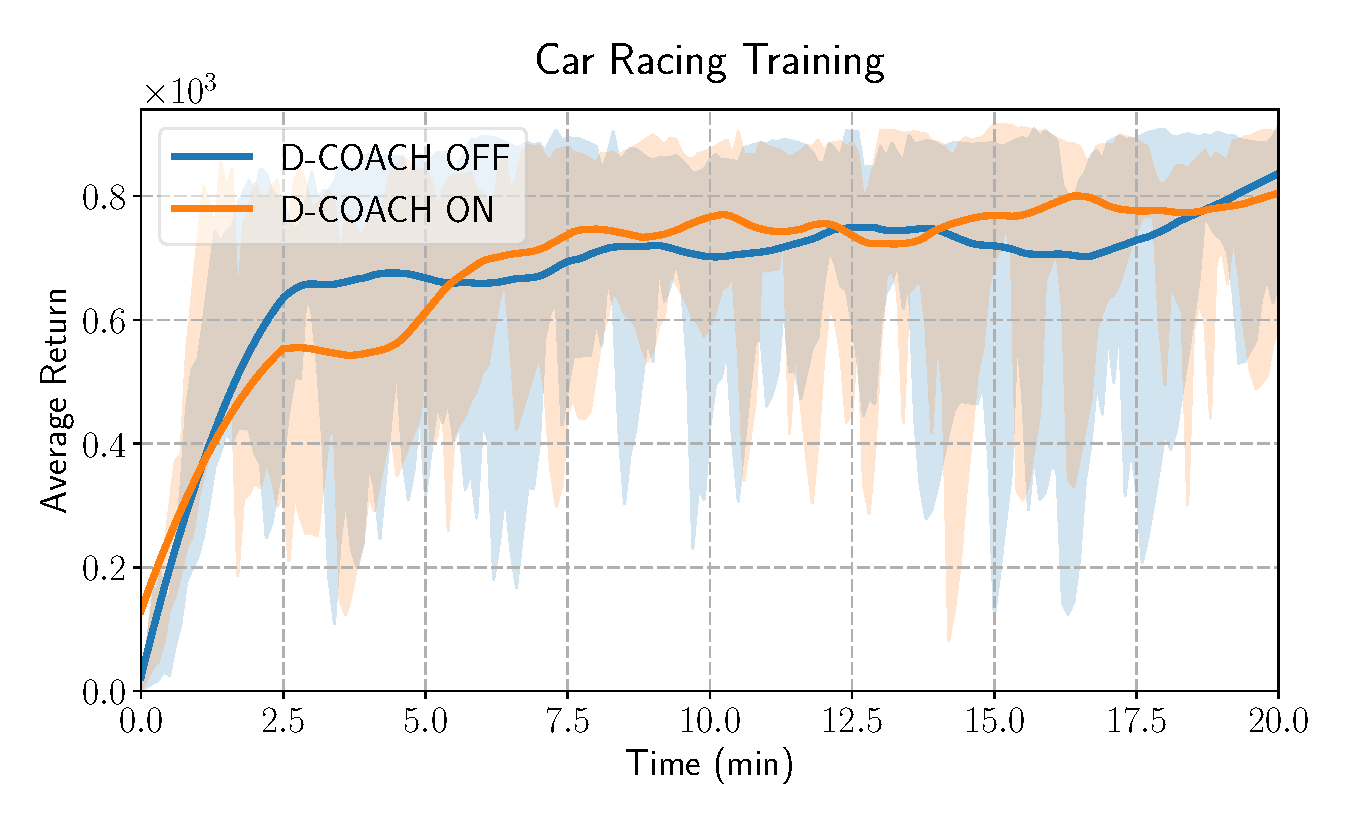
\includegraphics[width=0.7\linewidth]{imagenes/cap3/car_racing_human_teacher_ICRA.pdf}
    \caption[Results of learning with human teachers in the Car Racing problem.]{Results of learning with human teachers in the Car Racing problem. $K = 1000$; $k=20$; $b = 10$; $N = 8$; $\emph{e}=\textbf{1}$; $m=50$; $\epsilon=0.0011$. Human teacher network learning rate: $0.003$; Autoencoder learning rate: $0.003$.}
    \label{fig:humanteachers1}
\end{figure}

\begin{figure}[H]
    \centering
    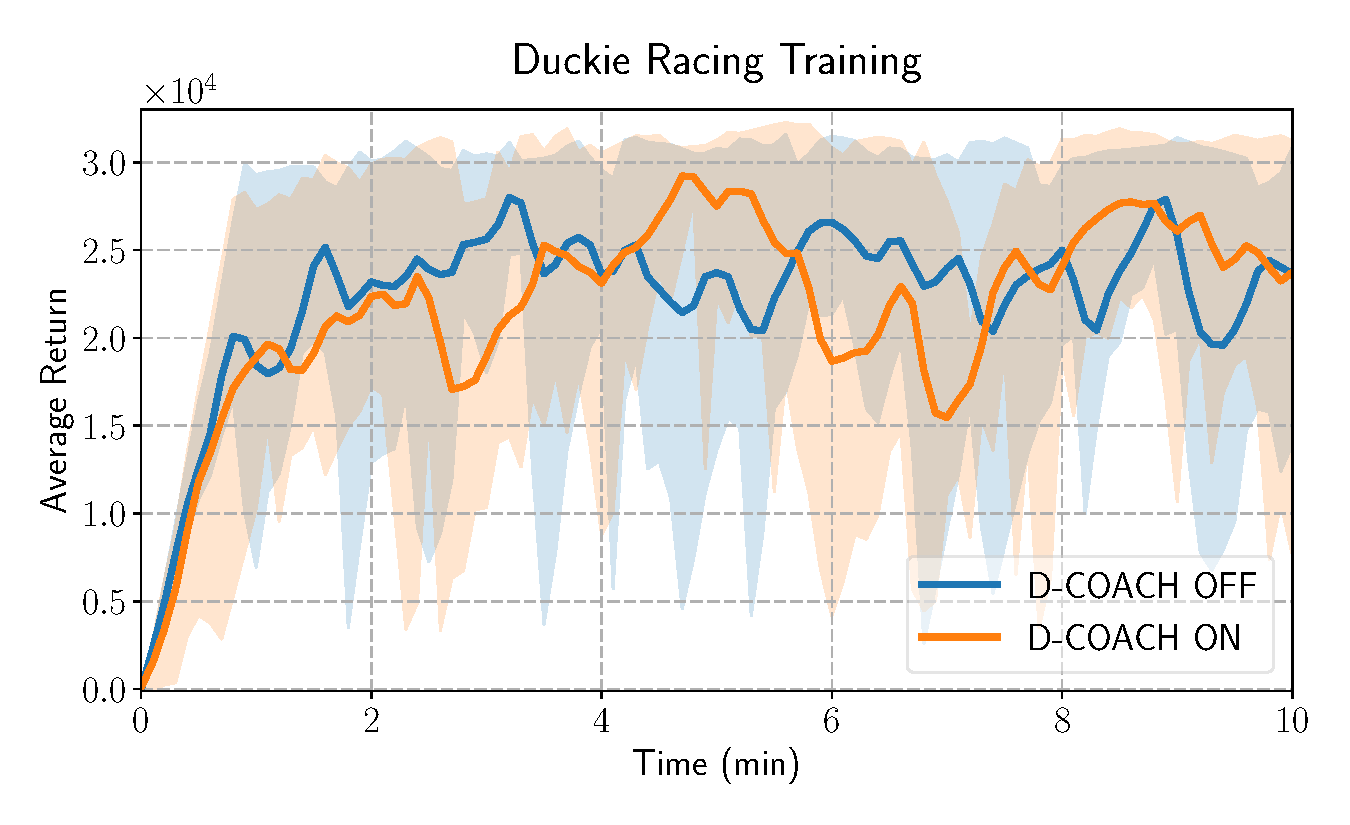
\includegraphics[width=0.7\linewidth]{imagenes/cap3/duckie_human_teacher_ICRA.pdf}
    \caption[Results of learning with human teachers in the Duckie Racing problem.]{Results of learning with human teachers in the Duckie Racing problem. $K = 1000$; $k=20$; $b = 10$; $N = 8$; $\emph{e}=\textbf{1}$; $m=50$; $\epsilon=0.0011$. Human teacher network learning rate: $0.003$; Autoencoder learning rate: $0.003$.}
    \label{fig:humanteachers2}
\end{figure}

\subsection{Additional validation with real systems}

Additional experiments with human teachers interacting with real robots through D-COACH ON were carried out. These tests are for validating the results obtained with the previous two types of experiments, and no comparisons are presented.

A real Duckiebot was used for validating the results obtained with the simulations. An experienced teacher advised the policy of Duckiebot from scratch and obtained a good policy in six minutes (experiment available in \url{https://youtu.be/i4f1D4CH26E}). Similarly, in the pusher/reacher problems well performing policies were obtained within twenty minutes. 

Fig.~\ref{fig:reacher_exp} shows an extra validation that was done for the reacher case. A cost function was defined as the Euclidean distance between the end-effector of the arm and the object to track, normalized with the largest possible distance within the image (distance of opposite corners). Seven training sessions of 15 minutes were run and averaged. It is possible to observe that the cost decreases as the learning process advances. 

\begin{figure}[H]
    \centering
    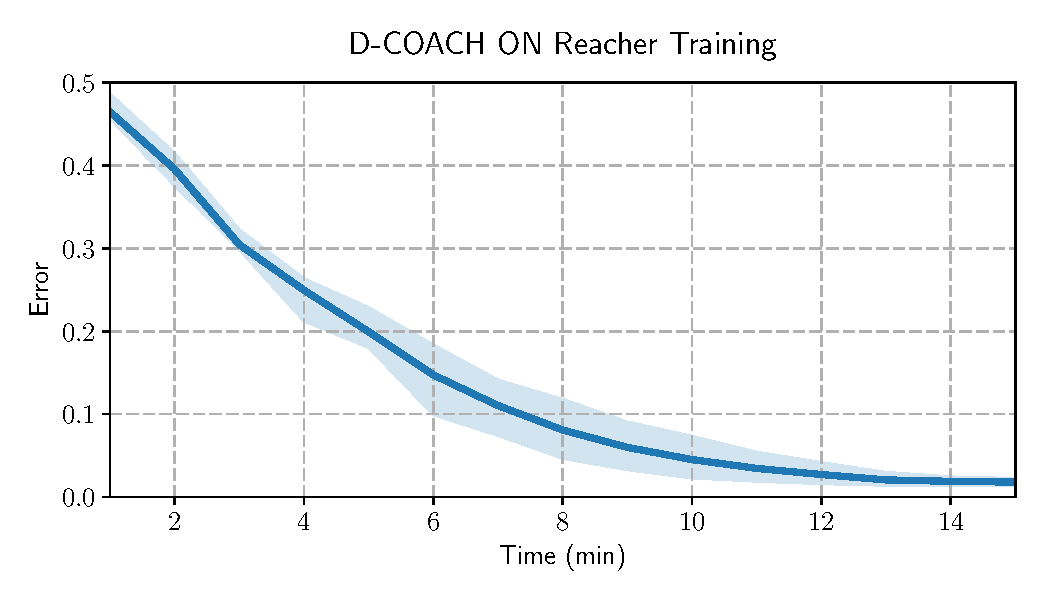
\includegraphics[width=0.7\linewidth]{imagenes/cap3/reacher_ICRA.pdf}
    \caption{Evolution of the error while learning the reacher task. }
    \label{fig:reacher_exp}
\end{figure}

\section{Discussion}

In this chapter we introduced an improved version of an interactive method for training policies represented with deep neural networks, particularly for problems wherein the observed state is defined in a high-dimensional space like a raw image.

The proposed D-COACH ON offers a simpler learning scheme of only one step in which state representation and the policy itself are learned jointly using the two optimization criteria (the AE cost and the regression error of the policy). This method eliminates the necessity of recording demonstrations for the pre-training of the AE, which is a time consuming effort for the user, and sometimes is not possible due to complexity of the problem and lack of complex skills of the user in the task domain. In the approached problems, the effort of the users was reduced between $45\%$ and $80\%$. D-COACH ON can adapt and extract features to represent reached unknown states during the learning process, which would be problematic for its basic version. Additionally, computational effort is reduced with the possibility of skipping the offline training of the AE, which is usually expensive. 

This simultaneous method is very data efficient for training the state representation. The AE is trained with the data gathered when human teachers advise corrections, which ensures a very representative database. Those samples correspond to the most important regions of the state space wherein the policy needs to discriminate different actions to execute.

The results also show that the interactive method can obtain higher performances than DDPG in very few episodes. The level of the performance achieved by the interactive method would be obtained by DDPG agents after several hundreds or thousands of episodes, which means that our proposed method is actually feasible, for learning with real robots in many applications wherein RL is not yet.